% Sample file on how to use subfiles.
\documentclass[ExampleMasters.tex]{subfiles}

\begin{document}
\clearpage
{\pagestyle{empty}\cleardoublepage}%
\chapter{Overview (6-7 Seiten)}
\label{chap:overview}


\section{Background of high capacity transport vehicles (HCT vehicles)}
\label{sec:legal_situation}
In this section first the legal regulations for \gls{HCT} vehicles in different countries are outlined, following that, the requirements for drivers of \gls{HCT} vehicles are described. After that, the impact of \gls{HCT} vehicles on the road infrastructure is looked upon.

In countries of the EU the permitted maximum length of a truck-trailer combination is 18.75 m and its maximum weight is 44 tonnes. There is however the possibility for countries to make exceptions from that rule.\cite{96/53/EC}  For example in Sweden and Finland road trains can be up to 25.25 m long with a  maximum weight of 60 tonnes.\cite{Vaegverket}
In several other countries of the EU \gls{HCT} vehicles are allowed on certain roads for testing purposes. 
Table \ref{tab:HCT_vehicles_in_different_countries} shows the maximum length and weight of \gls{HCT} vehicles in different countries.

\begin{table}[!htb]
	\centering
	\caption{\gls{HCT} vehicles in different countries\cite{Vaegverket}\cite{HCT_vehicles_Australia}\Cite{HCT_vehicles_USA}\cite{HCT_vehicles_Canada}\Cite{HCT_vehicles_Mexico}}
	\label{tab:HCT_vehicles_in_different_countries}
	\begin{tabular}{l|l|l|}
		Country   & Max. Length [m] & Max. Weight [t] \\ \hline
		EU (general) & 18.35 & 44.00\\
		Sweden    &       25.25      &       60.00      \\
		Finland   &            25.25 &         60.00    \\
		Australia &      53.50       &           132.00  \\
		USA(trailers without truck)&      26.07       &    59.86        \\
		Canada & 36.88 & 63.50 \\
		Mexico & 31.00 & 75.50 \\
	\end{tabular} \\
\end{table}
In Sweden there are attempts to have \gls{HCT} vehicles that exceed the current dimensions. One example is an A-double combination, which consists of a tractor, two semitrailers and a dolly between the semitrailers. This type of combination was used for the simulations and \gls{HIL} tests conducted in this project.\\

There are certain regulations for \gls{HCT} vehicles in terms of driver requirements. In countries of the European Union a person who drives a \gls{HCT} vehicles is required to have the CE class drivers license, which allows you to drive a tractor with a  mass over 3.5 tonnes with a trailer, whose mass is over 750 kg. To be able to acquire that drivers license the person has to be over 21 years old. \cite{EU_driving_licenses} 
On top of that, there have been more requirements for the drivers that took part in trials of \gls{HCT} vehicles in European countries. For example for the trials in the Netherlands drivers were required to have their drivers license for at least five years, to not have lost it during the last three years and they had to acquire a special certificate. To get that certificate the drivers had to take theoretical as well as practical courses.
\cite{HCT_vehicles_test_netherlands} \\

When it comes to the impact of road transport on road infrastructure, road wear is the most important effect. The main factor of road wear is the axle load of the vehicles. The following equation for a load equivalency factor shows how different axle loads impact road wear.   

\begin{equation}
\frac{N_{ref}}{N_x}=\left(\frac{W_x}{W_{ref}}\right)^4
\label{eq:LEF}
\end{equation}
Where $W_x$ and $W_{ref}$ are axle loads and $N_x$ and $N_{ref}$ are the corresponding numbers of load applications.\cite{road_wear} Equation \eqref{eq:LEF} shows that for example doubling the axle load leads to a road wear that is 16 times higher.

Assuming an equal distribution of the load over the different axles, the axle load for a vehicle is calculated as follows:\\
\begin{equation}
W_x=\frac{m_{tot}}{n_{axl}}
\label{eq:Axle_load}
\end{equation}
Where $m_{tot}$ is the total mass of the vehicle and $n_{axl}$ is the numbers of axles.
A standard tractor-semitrailer combination has five or six axles and a maximum mass of 40 tonnes.
With equation \eqref{eq:Axle_load} the axle load, if fully loaded, for that combination is 8 tonnes/axle and 6.67 tonnes/axle, respectively.
An A-double-combination, which has ten or eleven axles and a maximum mass of 80 tonnes, also reaches a maximum axle  load of 8 tonnes/axle and 7.27 tonnes/axle, respectively.
For a 25.25 m combination, which has nine or ten axles and a maximum mass of 60 tonnes, the maximum axle load is even lower than for the standard combination. The maximum axle load for this case is 6.67 tonnes/axle and 6 tonnes/axle, respectively.
\\Based on that it can be concluded that high capacity transport vehicles don't lead to higher road wear than standard combinations.


\section{Ongoing research}
\label{sec:ongoing_research}
There is a lot of research going on concerning high capacity transport vehicles. The main topics are the safety of \gls{HCT}, their environmental impact as well as economical aspects.\\

There are many concerns about the safety of \gls{HCT} in public opinion, so there have been quite a lot studies that investigated this issue. One concern is the extended length of \gls{HCT}, which causes an increase of time needed to overtake a combination. Studies showed that accident risk for overtaking a long combination is not statistically higher than for standard combinations \cite{EMS}.
For overall safety, the majority of studies show that the use of \gls{HCT} increases traffic safety due to the reduced number of vehicles on the roads, which is induced by the higher capacity of \gls{HCT} vehicles. However, \gls{HCT} might have a higher accident rate for individual vehicles \cite{EMS}. In another study crash data from the Swedish Traffic Accident Data Acquisition was analyzed. The results showed that there is no higher rate of fatal or severe crashes per traveled vehicle km for \gls{HCT} vehicles compared to standard vehicle combinations. \cite{balint2013correlation}

To reduce the effects on safety, which might occur with the use of \gls{HCT}, different safety systems are being developed.

One aim of safety systems for \gls{HCT} is to reduce the rearward amplification of yaw rate and lateral acceleration. A possibility to achieve that is to use a steerable dolly. In section \ref{sec:high-speed_controller} a controller to reduce rearward amplification for high speed is described.\\
Another problem of \gls{HCT} is the off-tracking of the last trailer for low speed cornering. Off-tracking means that the trailer doesn't follow the path of the tractor but moves on a radius that is smaller then the tractors. This issue can also be addressed by using a steerable dolly. In section \ref{sec:low-speed_controller} a controller to improve the path-following is described.

Since one of the reasons for using of \gls{HCT} vehicles is the expected positive influence on the environment compared to standard combinations, several studies that address this topic can be found.   
Overall this studies showed that with the use of \gls{HCT} vehicles the environmental impact of goods transportation can be reduced significantly for high loading factors. The fuel consumption is about 15\% lower compared to the standard vehicle combinations used in the EU. In the number of trips a reduction of 32\% can be seen. This reduction is achieved because two \gls{HCT} vehicles can carry the same amount of goods as three standard vehicle combinations.  \cite{backman2002improved}
However, the environmental impact of \gls{HCT} vehicles can become negative if due to a high penetration of \gls{HCT} vehicles goods transportation is shifted from rail to the road. \cite{doll2009long}

The introduction of new systems is alway driven by economical aspects, especially in the transportation industry. This \colorbox{yellow}{VBLBALLABLBA} \gls{HCT} vehicles is their economical advantage. First of all, the transport costs decrease by 1.8-3.4\%. Together with the environmental costs, that are lower compared to standard combinations, an overall benefit of \gls{HCT} vehicles can be seen.\cite{EMS}


\section{Market overview for existing solutions}
\label{sec:market_overview}
There are some solutions for dollys with steerable axles that exist today. However, the steering angles of the axles is only based on the articulation angle between the dolly and the trailer or truck it is attached to. \\
One of these solutions is the "active articulated dolly" manufactured by "Fahrzeugwerk Bernard Krone". The front axle of this dolly is steerable. In order to achieve that, the drawbar of the dolly is mechanically connected to the frontaxle and is rotateable. So if the drawbar is turned the wheels of the front axle steer. The transmission of the steering \gls{CAN} be varied by changing the length of the drawbar, which is adjustable. For safety reasons the steering is mechanically locked automatically depending on the velocity. The main reason for implementing this steering capability is to reduce off-tracking. This dolly is equipped with air suspension, an electronic breaking system as well as a stability system. \cite{Krone_dolly} \\
Other manufacturers that offer steerable dollys, that work the same way, are "Schmitz Cargobull" and "K{\"o}gel Trailer". \cite{Kogel_dolly}\cite{Schmitz_dolly} \\
In order to use the dolly to improve the vehicle dynamics of a  combination in a more advanced way, a solution that allows more independently steering is preferable. The dolly used in this project is capable of steering both front and rear axles individually and independent of the articulation angle between the dolly and the trailer in front of it. In section \ref{sec:dolly_system} this system is described in detail.


\section{Rapid Control Prototyping}
\label{sec:rapid_proto}

In automotive software development standardized processes are applied to assure structured work. The V-model which derives its name from the characteristic shape constitutes one graphic representations of the sequence of steps towards the finished overall system. It also gives an approximate impression about the level of detail of each of the steps on the vertical axle, as well as chronological progress on the horizontal. A simplified version of this V-model can be seen in figure \ref{fig:v_model}. First the user or customer needs are analyzed and put into a schematic formulation of the system showing the logic dependencies and underlying physical working principles. This is usually done in a semi-standardized fashion utilizing \gls{UML} or similiar diagrams, preventing non-specific prose to ensure less room for mis-communication and better readability. Technical decisions and limitations are not yet considered. After the logical system and dependencies have been established they will be analyzed and broken down to actual technical system descriptions defining also which subsystem will take over which function, what parts are to be realised as software or hardware (e.g. filtering, safety functions). The different parts of the technical system are then specified in detail, defining interfaces between different software sub-system, operational states and distribution of functions over sub-systems. The fourth step will define the specifications for the software in details for example: data types, control sequences, decision structures, real-time behaviour. Finally the actual design step will implement these specification with regards to the hardware limitations (RAM/ROM, processing power), computation methods, data handling (detailed format, variable types, utilization of parameters or variables). To compile the system from the component-level sub-system a similar hierachy is used in inverse. The corresponding steps of the project definition and specification phase (left side of the schematic) are supposed to provide test-procedures and goals. If necessary after insufficient test outcomes, another iteration of the previous step will be performed (vertical iterations). A similar sequence of development steps is applied to develop the hardware platform in parallel.\cite{automotive_software_engineering}

\begin{figure*}[!htb]
	\centering
	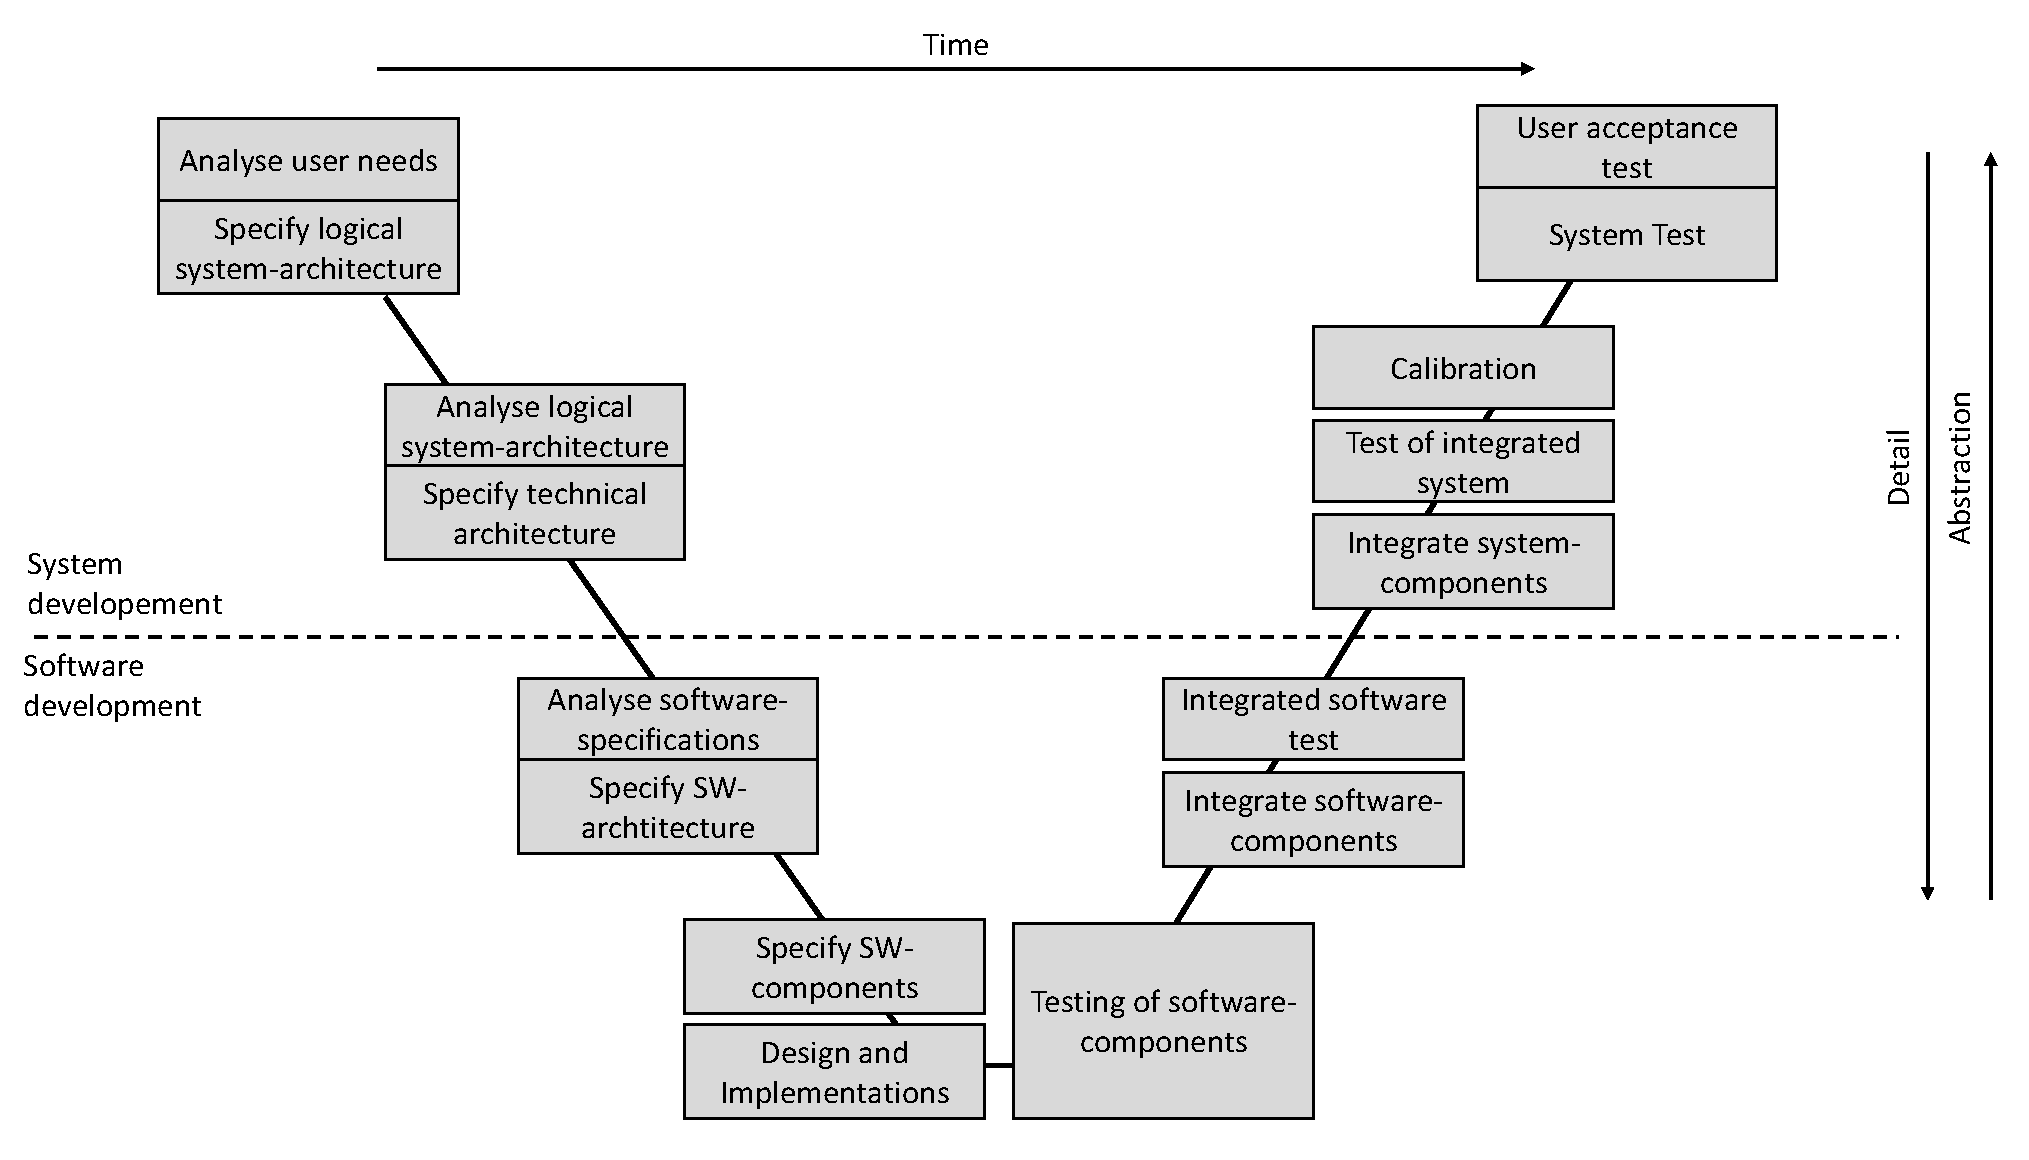
\includegraphics[width=0.9\linewidth]{figures/v_model/Folie1}
	\caption{Overview for a process in automotive software development after the V-model}
	\label{fig:v_model}
\end{figure*}



The increasing complexity of mechatronic systems and shorter product life-cycles lead to new development methods that made it possible to take 'short-cuts' in the established V-model process. This methods are summarized under the term rapid prototyping - in the case of software functions for mechatronic systems the term \gls{RCP} was coined. It is possible to conduct testing and verification with early soft- and hardware versions which are still under development by having the remaining system and environmental influences simulated by the \gls{RCP}-platform. In utilizing these methods such as rapid control prototyping and software/hardware-in-the-loop testing, a tremendous decrease in development time can be achieved. It is also possible to validate specifications early in the process, eliminating possible cost-intensive changes in later stages.\cite{rapidcontrolprototyping} For the research project in which this theses is embedded it even opens up the possibility of on-road testing, as it eliminates the low-level development steps of the actual implementation and some of the detailed design work. The implementation of the steering algorithm (see section \ref{chap:steering_model}) on a stand-alone ECU, hydraulic actuator control, hardware layout, etc. would by far exceed the dimensions of a research project. Applying rapid control prototyping is the only feasible way to establish a functioning on-road prototype vessel.


\begin{itemize}
	\item V-model
	\item real-time capability
	\item abstract high level model to programm ==> focus on function development and modelling, no low level coding needed
	\item time critical processes
	%\item extensive lecture notes from \cite{rapidcontrolprototyping}
\end{itemize}

\section{Functionality architecture}
\label{sec:func_architecture}

As a basis for this project a functionality architecture developed at Volvo GTT was used. The different parts of this architecture are shown in Figure \ref{fig:funct_architecture}.

\begin{figure*}[!htb]
	\centering
	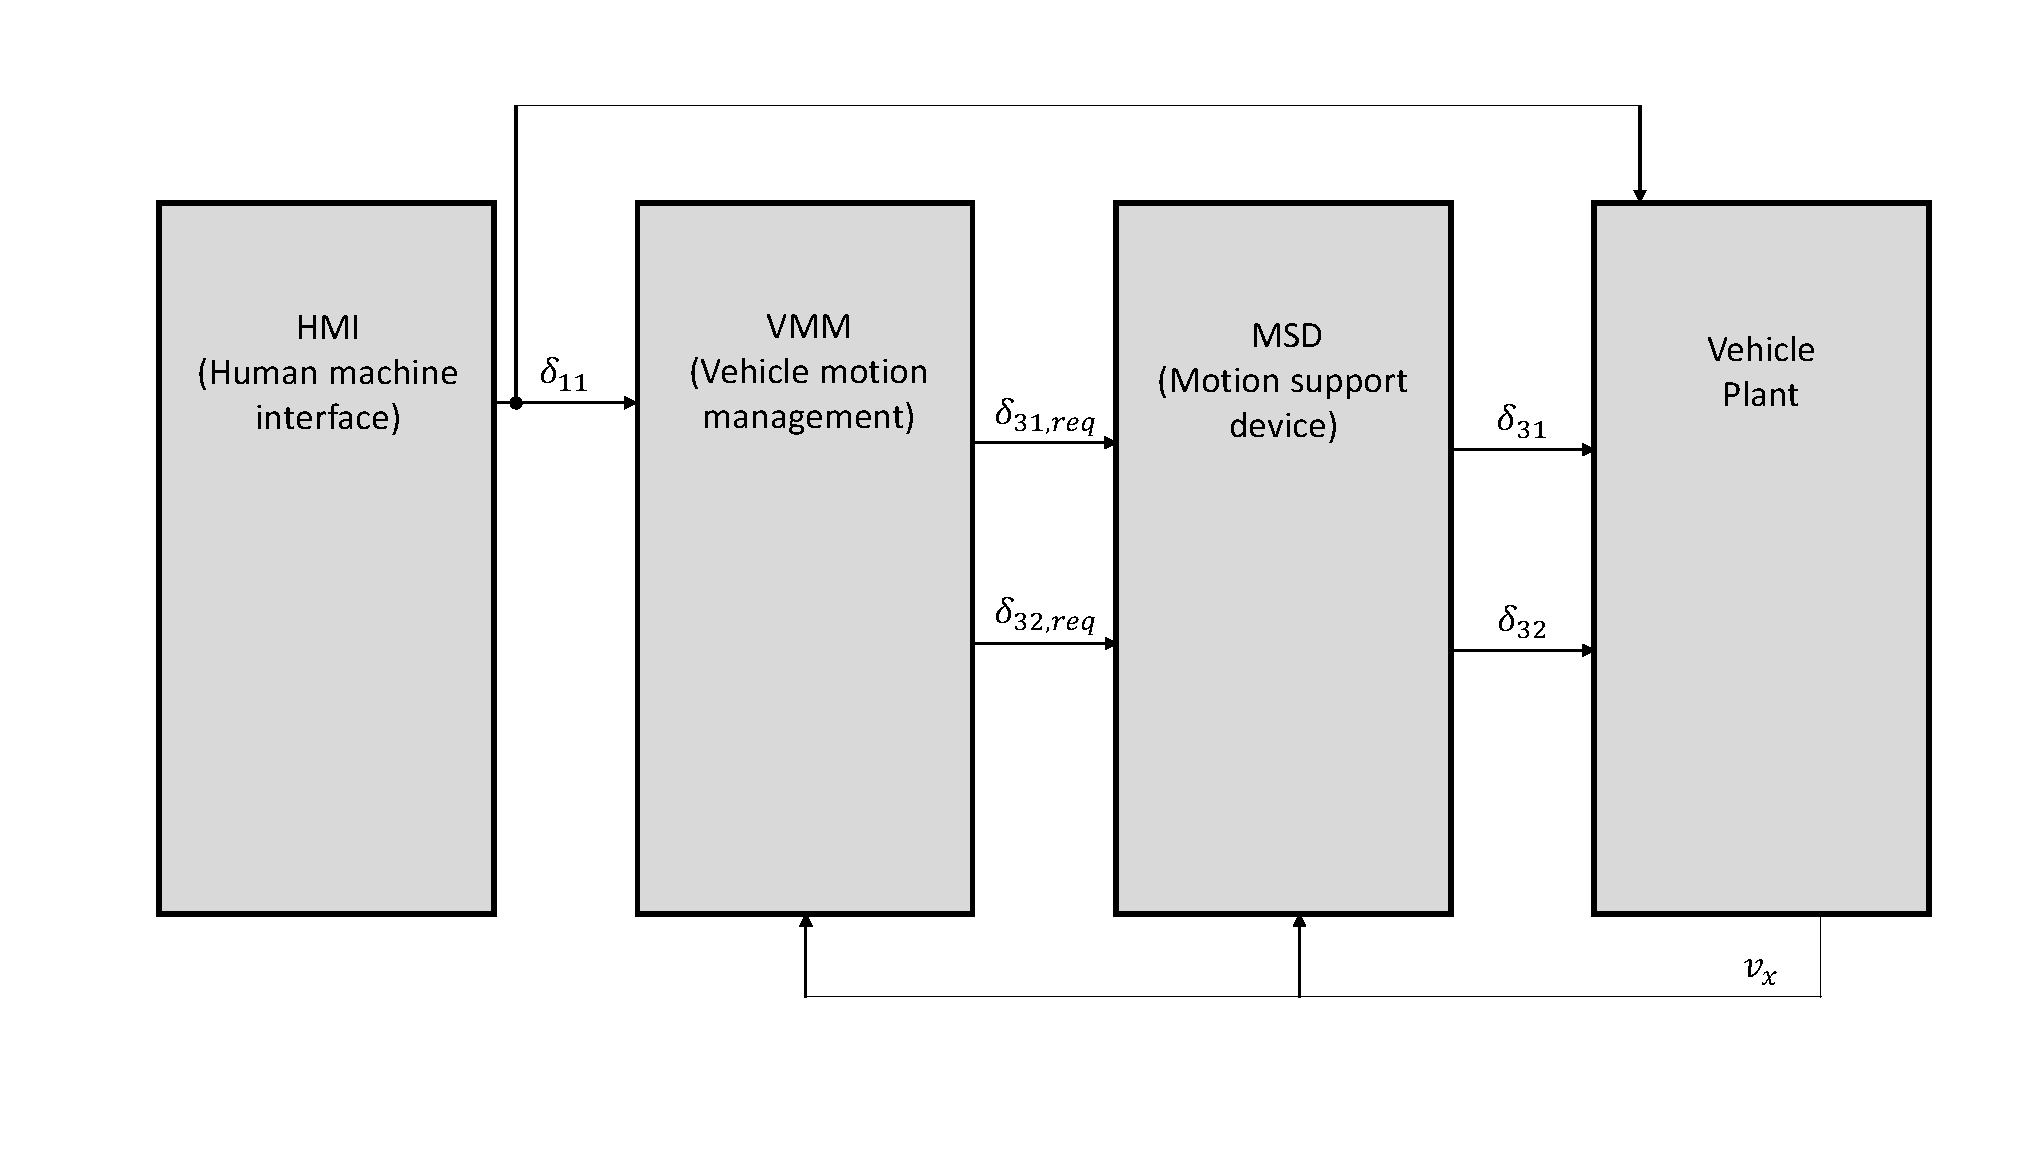
\includegraphics[width=1\linewidth]{figures/functionality_architecture}
	
	\caption{Functionality Architecture}
	\label{fig:funct_architecture}
\end{figure*}

The functionality architecture consists of four different parts: The Human machine interface, the vehicle motion management, the motion support devices and the vehicle plant.\\
The Human machine interface (HMI) is the interface between the driver and the vehicle. The driver can input requests to the vehicle, for example a steering angle via the steering wheel or a torque request via the accelerator pedal. The driver gets feedback from the vehicle about the vehicle's state, for example via the speedometer.

The vehicle motion management (VMM) contains the high-level controllers for the vehicle's motion and stability. It has an time horizon up to one second. As an input it gets the request of the driver from the HMI and transforms these requests into requests for the actuators of the vehicle. These request are then sent to the Motion support device (MSD). From the MSD the VMM receives information about the state of the actuators and the current capabilities.

The MSD contains the actuators and low-level controllers of the vehicle. In there the requests from the VMM are executed. Information about the status of the actuators is sent both to the VMM and the vehicle plant.

The vehicle plant corresponds to the rest of the vehicle.
\\
In different kind of tests, the parts of the functionality architecture are either simulated or real hardware is used. The more advanced the development process is, more and more of the functionality is shifted from simulation to actual hardware.




\end{document}
